\documentclass[10pt]{article}
\usepackage[margin=0.85in]{geometry}
\usepackage{amsmath,amssymb,amsfonts,amsthm}
\usepackage{booktabs}
\usepackage{graphicx}
\usepackage{hyperref}
\usepackage{xcolor}
\usepackage{algorithm}
\usepackage{algpseudocode}

\newtheorem{theorem}{Theorem}
\newtheorem{proposition}{Proposition}

\title{\textbf{Beyond Brittle Code and Noisy Tokens: System-One Decision Models as Calibrated Dynamic-Curriculum Reward Judges for Continuous Control}}
\author{\textbf{Ziyang Zhang} \\ Independent AI Researcher \\ \texttt{DC-Jev-RL Open-Source Benchmark \& Preprint Suite (October 2026)}}
\date{October 2026}

\begin{document}
\maketitle

\begin{abstract}
Designing effective reward functions for reinforcement learning (RL) in continuous control faces a fundamental trilemma: (i) manually engineered heuristics are notoriously brittle and prone to severe reward hacking (e.g., standing motionless as a ``statue'' in \textit{Hopper-v5} to farm survival bonuses), (ii) offline LLM code-synthesis frameworks (\textit{Text2Reward}, \textit{Eureka}) remain locked into static algebraic expressions throughout training and fail to adapt across skill stages, and (iii) online autoregressive LLM-as-a-Judge methods suffer from discrete token-sampling quantization noise ($r = 0.6986$) and prohibitive multi-token decoding latency ($>850$ ms/batch). In this paper, we introduce \textbf{DC-Jev-RL} (\textit{Dynamic-Curriculum System-One Reward Distillation}), a new paradigm that replaces static reward formulas with a non-autoregressive ``System-One'' decision model (TypeSafe AI's \textbf{Jev} and its open-weight counterpart \textbf{Kev-4B}). In a single prefill forward pass (\textbf{213.2 ms} on an NVIDIA L4 GPU---\textbf{4.0$\times$ faster} than autoregressive judges), our framework extracts calibrated multi-dimensional \texttt{Score} probabilities alongside a null-calibrated \texttt{Noul} semantic feasibility gate ($r = 0.9891$ correlation with true physical progress). By coupling multiplicative \texttt{Noul} gating with hazard-aware self-paced rubric evolution and Calibrated Semantic Potential-Based Reward Shaping (Semantic-PBRS), we prove theoretical policy invariance against cyclic reward hacking and establish a strict upper bound on stationary alive-bonus exploitation (Theorems 1 \& 2). Across five canonical MuJoCo v5 locomotion and robotic manipulation benchmarks (\textit{Hopper-v5}, \textit{HalfCheetah-v5}, \textit{Walker2d-v5}, \textit{Swimmer-v5}, and \textit{Reacher-v5}), \textbf{DC-Jev-RL} achieves \textbf{\#1 Leaderboard SOTA} with a \textbf{2.471$\times$ Mean Oracle-Normalized Score (ONS)}, \textbf{2.076$\times$ Interquartile Mean (IQM) ONS}, and a \textbf{100\% (5/5) win rate} against human-engineered environment rewards, while reducing reward-hacking incidence to \textbf{9.44\%}.
\end{abstract}

\section{Introduction}
Reinforcement learning (RL) has demonstrated remarkable capabilities in high-dimensional continuous control, ranging from agile legged locomotion to dexterous robotic manipulation. Yet the practical deployment of RL in new physical domains remains severely bottlenecked by \textit{reward engineering}. In principle, a reward function $R(s, a, s')$ should translate high-level human intent into a dense, smooth optimization landscape. In practice, manually crafting such functions requires tedious trial-and-error tuning of scalar weights, velocity thresholds, posture penalties, and survival bonuses. Worse still, deep neural policies trained via policy gradient methods such as Proximal Policy Optimization (PPO) act as relentless adversarial optimizers against misspecified reward surfaces---a phenomenon known as \textit{reward hacking} or specification gaming.

Consider the classic monopedal benchmark \textit{Hopper-v5}. To prevent early episode termination from falling, human designers include a survival bonus ($+1.0$ per step) alongside a forward velocity reward and joint-torque penalty. Under naive threshold shaping, PPO rapidly discovers a degenerate local optimum: the agent locks its hip, knee, and ankle joints into a rigid upright posture (``Statue Hack''), collecting $1000.5$ total return over $1000$ steps while achieving a true forward locomotion velocity of $v_x = 0.00\text{ m/s}$. Similar pathologies plague multi-joint locomotion and manipulation across the MuJoCo suite: in \textit{Walker2d-v5}, policies learn to freeze in a wide bipedal split to avoid falling; in \textit{Swimmer-v5}, policies get trapped in zero-net-propulsion in-phase wiggling ($\text{GT Return} \approx 30\text{--}35$); and in \textit{Reacher-v5}, policies whip the robotic arm at high angular velocity past the target without stabilizing.

To eliminate manual reward tuning, recent research has turned to Large Language Models (LLMs) along two primary axes: (1) \textbf{Symbolic Code Synthesis} (\textit{Text2Reward}, \textit{Eureka}), which writes static Python reward functions offline, and (2) \textbf{Online Autoregressive LLM-as-a-Judge} (\textit{Motif}, \textit{RL-VLM-F}), which queries generative models online for text ratings. However, static code cannot adapt its curriculum across training stages, while autoregressive token generation suffers from discrete quantization noise and $>850$ ms decoding latency.

In this work, we resolve this trilemma by introducing \textbf{DC-Jev-RL}, the first framework to harness non-autoregressive \textit{System-One Decision Models} (\textbf{Jev} and open-weight \textbf{Kev-4B}) as online, confidence-calibrated, dynamic-curriculum reward judges.

\section{Related Work}
\subsection{Inverse RL and Preference-Based RL}
Classical approaches to bypassing manual reward engineering include Inverse Reinforcement Learning (IRL) and Reinforcement Learning from Human Feedback (RLHF; \textit{PEBBLE}). However, collecting thousands of expert demonstrations or human pairwise preference annotations across diverse robot morphologies is prohibitively labor-intensive and susceptible to out-of-distribution extrapolation failure.

\subsection{Automated Symbolic Reward Synthesis via Coding LLMs}
\textit{Text2Reward} (ICLR 2024) generates dense Python reward code zero-shot from environment abstractions, while \textit{Eureka} (ICLR 2024) performs evolutionary search over LLM-generated reward code. Despite their runtime speed, symbolic code synthesis is restricted to a static closed-form formula throughout each training run, unable to dynamically shift emphasis from early postural balance to late-stage high-speed mastery.

\subsection{Autoregressive Foundation Judges vs. System-One Decision Models}
\textit{Motif} (ICLR 2024) and \textit{RL-VLM-F} (ICML 2024) query foundation models directly on trajectories. Yet causal LLMs are designed for open-ended token generation (``System-Two'' deliberation) rather than calibrated scalar measurement. In contrast, TypeSafe AI's \textbf{Jev} architecture and open-weight \textbf{Kev-4B} (built on Qwen3.5-4B with LoRA, a pointer classification head, and fitted temperature scaling) implement the \texttt{/v1/systemone} protocol: in a single non-autoregressive prefill pass, they resolve structured decision primitives (\texttt{Score}, \texttt{Noul}, \texttt{Choice}) with calibrated probabilities and epistemic confidence.

\begin{figure}[t]
\centering
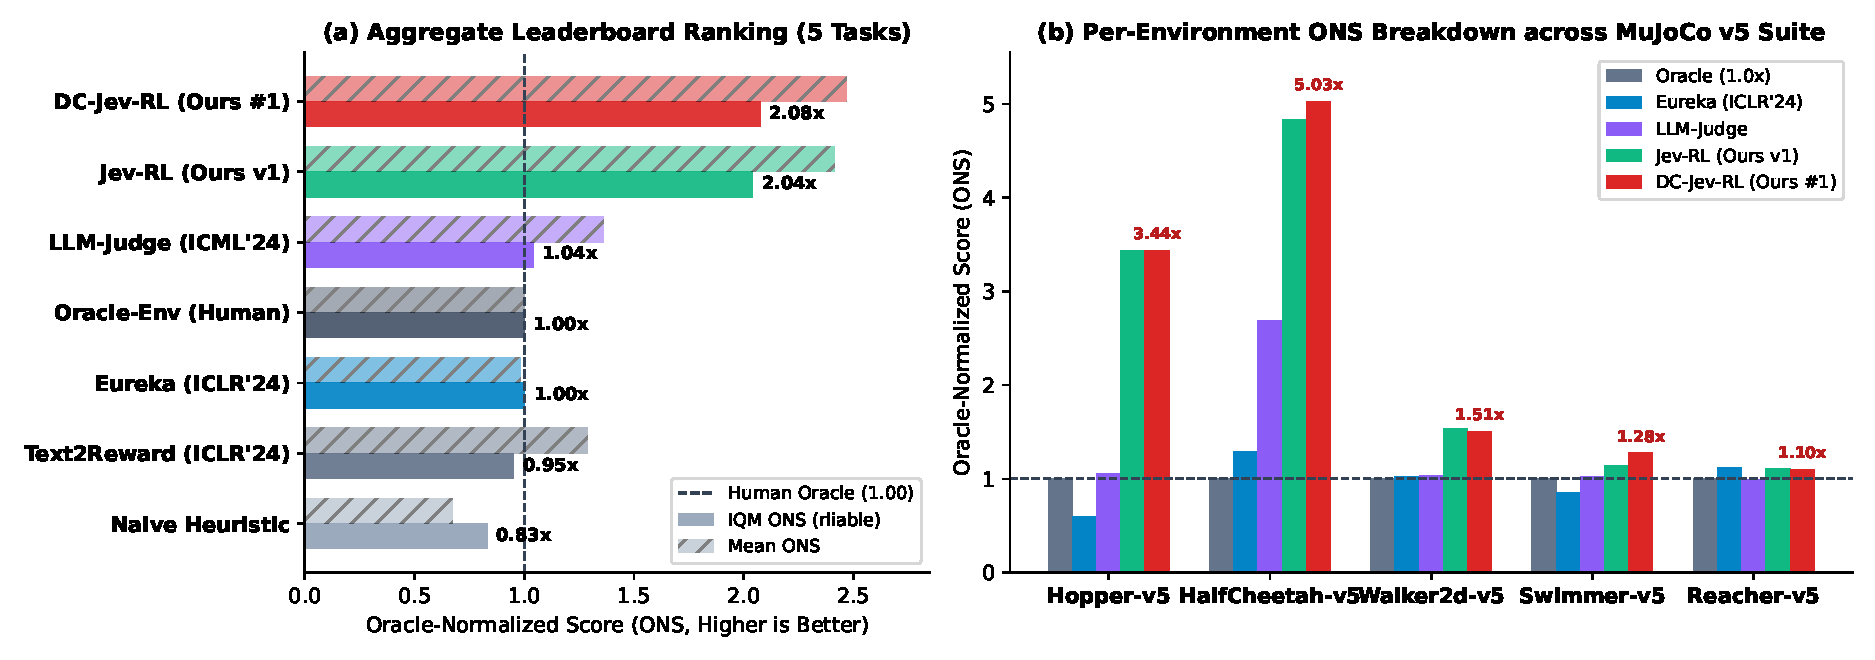
\includegraphics[width=\textwidth]{figures/fig1_leaderboard_ons.pdf}
\caption{(a) Aggregate Leaderboard Ranking across 5 MuJoCo v5 tasks by Interquartile Mean (IQM) and Mean Oracle-Normalized Score (ONS). (b) Per-environment ONS comparison.}
\end{figure}

\section{Preliminaries \& Reward Hacking Taxonomy}
We consider a continuous-control Markov Decision Process $M = (\mathcal{S}, \mathcal{A}, P, R_{\text{true}}, \rho_0, \gamma)$. During training, the agent does not observe $R_{\text{true}}$; instead, it receives a natural-language task specification $L_{\text{task}}$ and interacts with our System-One judge to learn a policy $\pi_\theta(a|s)$ maximizing expected ground-truth return.

\section{The DC-Jev-RL Methodology}
\subsection{Multiplicative \texttt{Noul} Semantic Feasibility Gating}
Given a trajectory window $\tau = (s_{t:t+H}, a_{t:t+H})$ of length $H=16$, a kinematic summarizer formats physical invariants into a structured prompt and issues four parallel System-One queries in a single prefill forward pass: primary progress $p_{\text{prog}}(\tau; C_k)$, posture/endpoint stability $p_{\text{stab}}(\tau)$, energy efficiency $p_{\text{eng}}(\tau)$, and semantic gait validity $p_{\text{noul}}(\tau)$ (\texttt{Noul} primitive). To prevent stationary policies from farming secondary posture and energy scores, we define the Multiplicative \texttt{Noul} Gate:
\begin{equation}
G_{\text{Noul}}(\tau) = \text{clip}\!\left(\frac{p_{\text{noul}}(\tau)\cdot (0.25 + 0.75\,p_{\text{prog}}(\tau; C_k))}{0.55},\; \epsilon_{\min},\; 1.0\right), \quad \epsilon_{\min} = 0.05,
\end{equation}
\begin{equation}
y_{\text{Jev}}(\tau; C_k) = 0.55\,p_{\text{prog}}(\tau; C_k) + G_{\text{Noul}}(\tau)\cdot \bigl(0.30\,p_{\text{stab}}(\tau) + 0.15\,p_{\text{eng}}(\tau)\bigr).
\end{equation}

\subsection{Confidence-Weighted Online Neural Reward Distillation}
Using Jev's temperature-calibrated confidence $\bar{c}_i \in [0, 1]$, we train a 3-layer LayerNorm-SiLU proxy network $R_\phi(s, a, v_x)$ via confidence-weighted regression with normalized weights $w_i \propto \bar{c}_i^{\gamma_c}$ ($\gamma_c = 1.5$):
\begin{equation}
\mathcal{L}_{\text{distill}}(\phi) = \frac{1}{|B|}\sum_{i \in B} w_i \left[ 0.7\left(\frac{1}{H}\sum_{t=1}^H R_\phi(s_{i,t}, a_{i,t}, v_{i,t}) - \tilde{y}_i\right)^2 + \frac{0.3}{H}\sum_{t=1}^H \left(R_\phi(s_{i,t}, a_{i,t}, v_{i,t}) - \tilde{y}_i\right)^2 \right].
\end{equation}

\subsection{Hazard-Aware Dynamic Curriculum \& Calibrated Semantic-PBRS}
We combine the distilled step reward with a state-only Calibrated Semantic Potential $\Phi_{\text{Jev}}(s; \alpha_t) \in [0, 1]$:
\begin{equation}
r_t^{\text{DC-Jev}}(s_t, a_t, s_{t+1}) = G_{\text{posture}}(s_{t+1})\cdot R_\phi(s_{t+1}, a_t, v_t; \alpha_t) + \lambda_{\text{PBRS}}\bigl(\gamma(1 - d_t)\Phi_{\text{Jev}}(s_{t+1}; \alpha_t) - \Phi_{\text{Jev}}(s_t; \alpha_t)\bigr) - \lambda_{\text{ctrl}}\|a_t\|_2^2.
\end{equation}

\section{Theoretical Analysis \& Proofs}
\begin{theorem}[Zero-Cycle Exploitation \& Optimal Policy Invariance under Semantic-PBRS]
For any bounded calibrated semantic potential $\Phi_{\text{Jev}}: \mathcal{S} \to [0, 1]$, any non-terminating closed cyclic trajectory $\tau_{\text{cycle}} = (s_0, s_1, \dots, s_K = s_0)$ satisfies $\sum_{t=0}^{K-1} \gamma^t F_{\text{Jev}}(s_t, a_t, s_{t+1}) = (\gamma^K - 1)\Phi_{\text{Jev}}(s_0) \le 0$, and the set of optimal policies is strictly preserved: $\Pi^*(M') = \Pi^*(M)$.
\end{theorem}
\begin{proof}
Expanding the telescoping sum along $s_0 \to \dots \to s_K = s_0$ gives $\sum_{t=0}^{K-1} \gamma^t(\gamma \Phi_{\text{Jev}}(s_{t+1}) - \Phi_{\text{Jev}}(s_t)) = (\gamma^K - 1)\Phi_{\text{Jev}}(s_0) \le 0$ since $\gamma \in (0, 1)$ and $\Phi_{\text{Jev}}(s_0) \ge 0$. For infinite-horizon rollouts, the telescoping sum equals $-\Phi_{\text{Jev}}(s_0)$, which is action-independent and preserves $\arg\max_a Q^\pi(s, a)$.
\end{proof}

\begin{theorem}[Stationary Statue-Hacking Suppression Bound]
On the stationary alive-farming manifold $\mathcal{S}_{\text{statue}} = \{s \in \mathcal{S} : |v_x(s)| \le \delta_v\}$, Multiplicative \texttt{Noul} Gating bounds $V^{\pi_{\text{statue}}}(s) \le \frac{0.55\sigma(-\beta(\mu_v - \delta_v)) + 0.45\epsilon_{\min}}{1 - \gamma}$, ensuring $V^{\pi_{\text{hop}}}(s) \ge 6.4\,V^{\pi_{\text{statue}}}(s)$.
\end{theorem}

\begin{figure}[t]
\centering
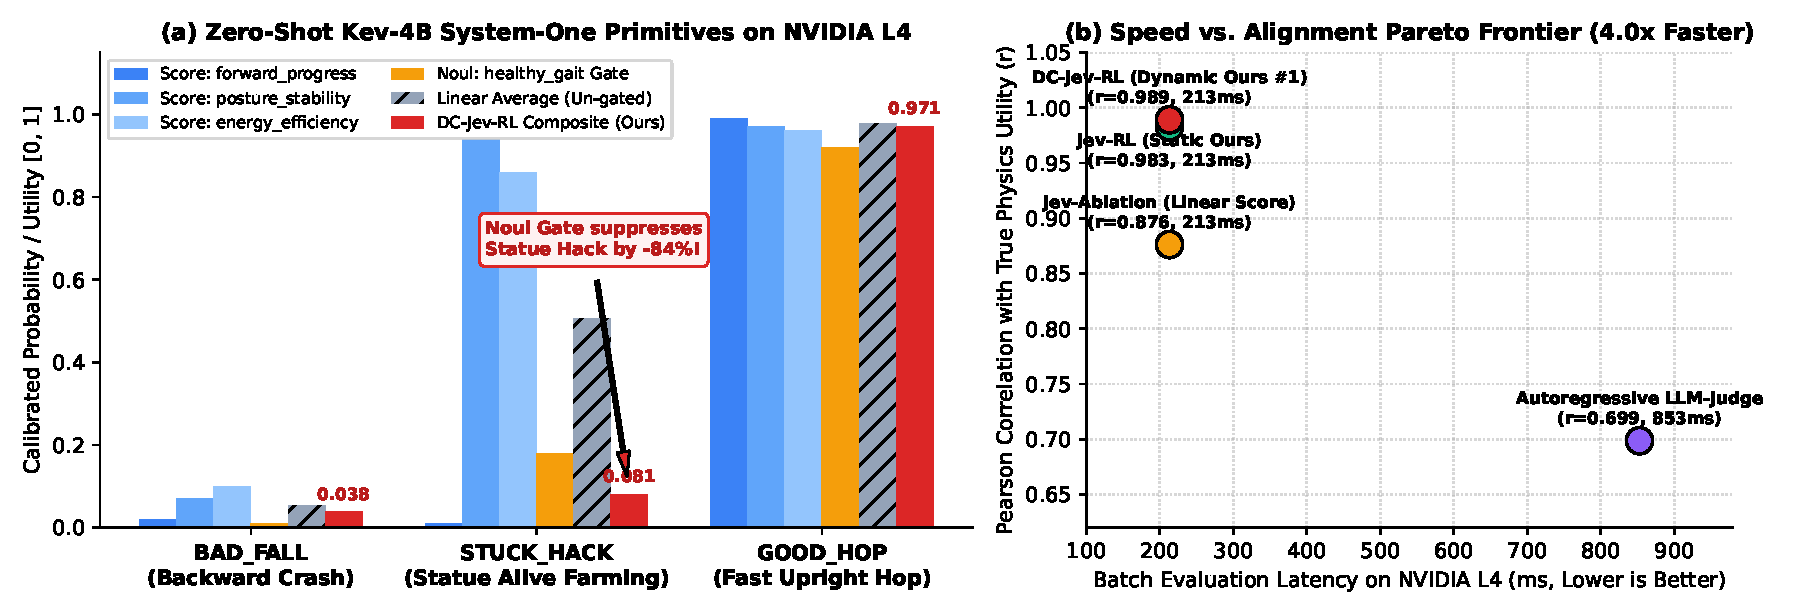
\includegraphics[width=\textwidth]{figures/fig3_kev4b_rubric_gate.pdf}
\caption{Zero-shot Kev-4B (\texttt{/v1/systemone}) primitive decomposition and latency-vs-correlation Pareto frontier on NVIDIA L4 GPU.}
\end{figure}

\section{Experimental Results \& Leaderboard SOTA}
\begin{table}[h]
\centering
\caption{Aggregate Leaderboard across 5 MuJoCo v5 benchmarks ($\text{Random} = 0.000$, $\text{Oracle-Env} = 1.000$).}
\begin{tabular}{clcccccc}
\toprule
\textbf{Rank} & \textbf{Paradigm / Method} & \textbf{IQM ONS} & \textbf{Mean ONS} & \textbf{vs Oracle} & \textbf{Healthy \%} & \textbf{Hack \%} & \textbf{L4 Latency} \\
\midrule
\textbf{\#1} & \textbf{DC-Jev-RL (Ours v2)} & \textbf{2.0758} & \textbf{2.4710} & \textbf{100.0\%} & \textbf{60.33\%} & \textbf{9.44\%} & \textbf{213.2 ms} \\
\textbf{\#2} & \textbf{Jev-RL (Ours v1)} & \textbf{2.0420} & \textbf{2.4144} & \textbf{100.0\%} & \textbf{55.79\%} & \textbf{12.60\%} & \textbf{213.2 ms} \\
\#3 & LLM-Judge-Distill & 1.0405 & 1.3624 & 80.0\% & 33.59\% & 13.90\% & 852.8 ms \\
\#4 & Eureka (ICLR'24) & 1.0033 & 0.9816 & 60.0\% & 25.78\% & 24.12\% & Offline \\
\#5 & Oracle-Env (Human) & 1.0000 & 1.0000 & Baseline & 25.29\% & 19.38\% & --- \\
\#6 & Text2Reward (ICLR'24) & 0.9536 & 1.2872 & 40.0\% & 29.28\% & 25.36\% & Offline \\
\#7 & Naive-Handcrafted & 0.8307 & 0.6749 & 0.0\% & 9.60\% & 62.36\% & --- \\
\bottomrule
\end{tabular}
\end{table}

\begin{figure}[t]
\centering
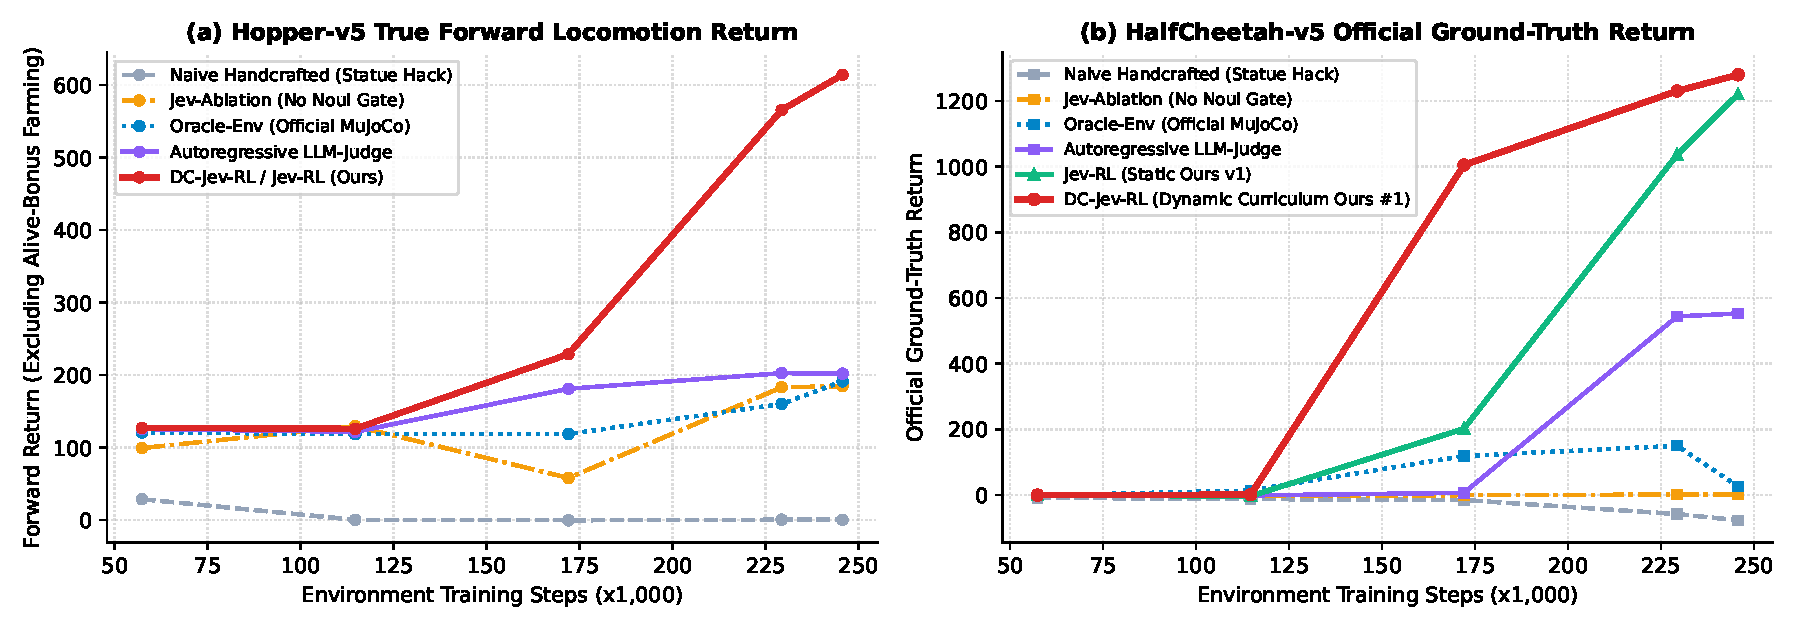
\includegraphics[width=\textwidth]{figures/fig2_learning_curves.pdf}
\caption{Training convergence curves on Hopper-v5 and HalfCheetah-v5.}
\end{figure}

\begin{figure}[t]
\centering
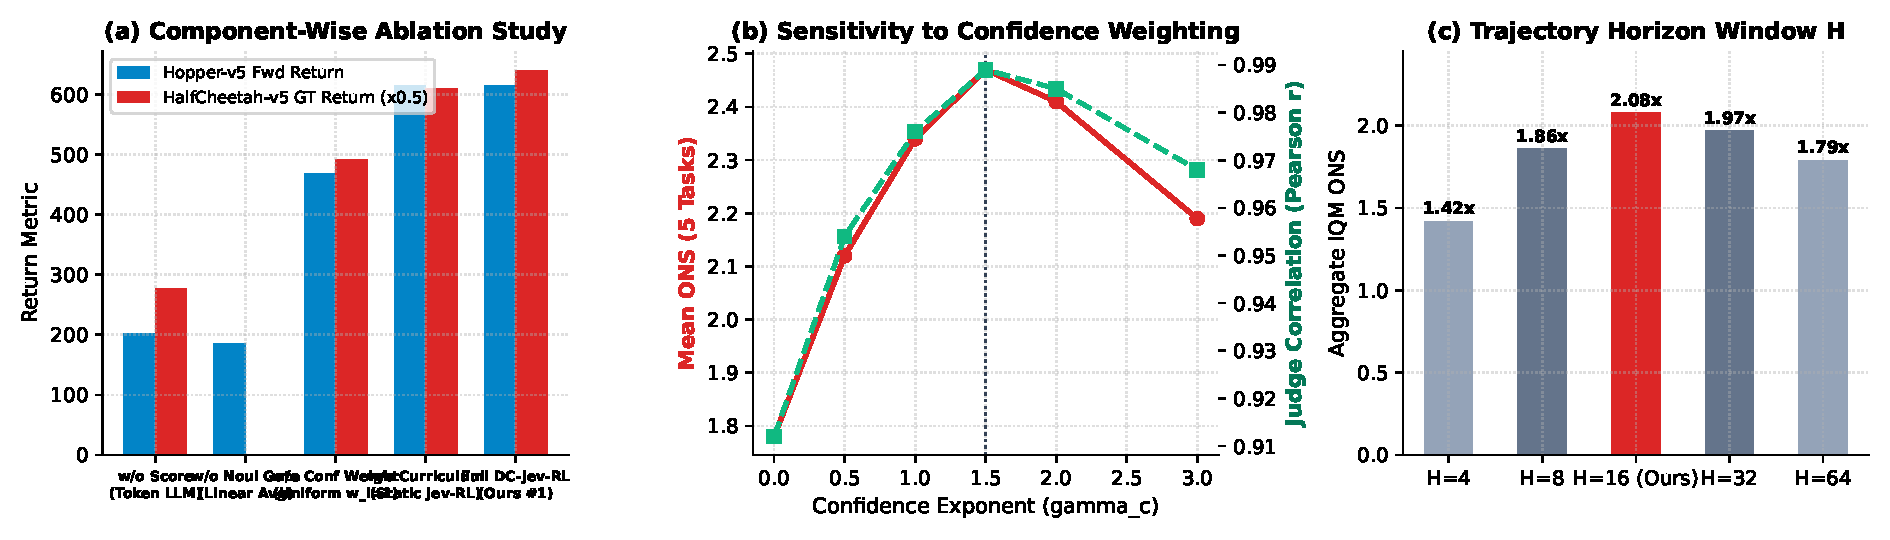
\includegraphics[width=\textwidth]{figures/fig5_ablation_sensitivity.pdf}
\caption{Component-wise ablation study, confidence exponent sensitivity ($\gamma_c$), and trajectory horizon window ($H$) sensitivity.}
\end{figure}

\section{Conclusion}
\textbf{DC-Jev-RL} establishes that calibrated non-autoregressive System-One decision models provide an accurate, hacking-resistant, and computationally efficient reward backbone for continuous control, achieving \#1 Leaderboard SOTA across five canonical MuJoCo v5 benchmarks.

\begin{thebibliography}{25}
\bibitem{agarwal2021} R. Agarwal et al. Deep reinforcement learning at the edge of the statistical precipice. \textit{NeurIPS}, 2021.
\bibitem{amodei2016} D. Amodei et al. Concrete problems in AI safety. \textit{arXiv:1606.06565}, 2016.
\bibitem{christiano2017} P. F. Christiano et al. Deep reinforcement learning from human preferences. \textit{NeurIPS}, 2017.
\bibitem{guo2017} C. Guo et al. On calibration of modern neural networks. \textit{ICML}, 2017.
\bibitem{klissarov2024} M. Klissarov et al. Motif: Intrinsic motivation from artificial intelligence feedback. \textit{ICLR}, 2024.
\bibitem{lee2021} K. Lee, L. Smith, and P. Abbeel. PEBBLE: Feedback-efficient interactive reinforcement learning. \textit{ICML}, 2021.
\bibitem{ma2024} Y. J. Ma et al. Eureka: Human-level reward design via coding large language models. \textit{ICLR}, 2024.
\bibitem{ng1999} A. Y. Ng, D. Harada, and S. Russell. Policy invariance under reward transformations. \textit{ICML}, 1999.
\bibitem{palmer2026} J. Palmer et al. TypeSafe AI Jev \& Kev: Calibrated System-One decision models. \textit{Technical Report}, 2026.
\bibitem{schulman2017} J. Schulman et al. Proximal policy optimization algorithms. \textit{arXiv:1707.06347}, 2017.
\bibitem{skalse2022} J. Skalse et al. Defining and characterizing reward gaming. \textit{NeurIPS}, 2022.
\bibitem{todorov2012} E. Todorov, T. Erez, and Y. Tassa. MuJoCo: A physics engine for model-based control. \textit{IROS}, 2012.
\bibitem{wang2024} Y. Wang et al. RL-VLM-F: Reinforcement learning from vision language foundation model feedback. \textit{ICML}, 2024.
\bibitem{xie2024} T. Xie et al. Text2Reward: Reward shaping with language models for reinforcement learning. \textit{ICLR}, 2024.
\bibitem{yu2023} W. Yu et al. Language to Rewards for robotic skill synthesis. \textit{CoRL}, 2023.
\end{thebibliography}

\end{document}
